\documentclass[11pt,a4paper]{article}

% ---------- Packages ----------
\usepackage[T1]{fontenc}
\usepackage{lmodern}
\usepackage[margin=1in]{geometry}
\usepackage{setspace}
\usepackage{textcomp} % for \pounds
\usepackage{graphicx}
\graphicspath{{assets/fair/}} % <-- where your publication-bundled PNGs live
\usepackage{booktabs}
\usepackage{siunitx}
\usepackage{hyperref}
\usepackage{caption}
\usepackage{subcaption}
\usepackage{float}

% ---------- Formatting ----------
\onehalfspacing
\sisetup{
  detect-all,
  group-separator = {,},
  group-minimum-digits = 4
}

\title{\textbf{Home@ix FAIR: A Forward Indicator of UK Housing Affordability Regimes Using Credit--Price Decoupling and Market Depth}}
\author{Home@ix (Working Paper / Draft)}
\date{25 February 2026}

\begin{document}
\maketitle

\begin{abstract}
UK housing affordability is usually discussed as a price level or a price-to-income ratio. That framing is necessary but incomplete because UK housing markets often do not clear primarily through price adjustment. In stressed regimes, markets clear through quantities and composition: turnover collapses, chains fail, mortgage-dependent households are rationed out, and observed prices can appear sticky or misleading. This paper introduces Home@ix FAIR: a quarterly indicator designed as a 2--3 year forward regime signal for affordability understood as access and allocation, not only price burden. FAIR is intentionally reduced-form and reproducible. It integrates a credit--price wedge (prices outrunning mortgage-stock growth), a market-depth term (turnover dynamics) capturing thin-market clearing, and an optional composition term (new-build share dynamics). To avoid defining ``normal'' using crisis regimes and structural breaks, FAIR is normalised to pooled baseline windows excluding the Global Financial Crisis aftermath and Covid-era disruptions. FAIR is paired with a direction-of-flow statistic and can be evaluated via event-based backtesting (drawdown-defined crash starts). Together, the index and backtests form an operational toolkit for monitoring affordability regime risk.
\end{abstract}

\section{Executive Summary}
UK housing affordability is typically treated as a static burden ratio. Yet housing is not a frictionless market. When credit tightens or uncertainty rises, the UK housing market frequently clears via reduced participation rather than orderly repricing: transactions fall, turnover collapses, and access deteriorates even when price ratios appear stable.

This paper introduces \textbf{Home@ix FAIR}, a reproducible quarterly indicator designed to act as a \textbf{2--3 year forward regime signal} for affordability understood as \textbf{access and allocation}. FAIR integrates:
\begin{itemize}
  \item a \textbf{credit--price wedge} capturing decoupling between house-price growth and mortgage-stock growth;
  \item a \textbf{market-depth / turnover term} capturing thin-market (quantity-clearing) stress; and
  \item an \textbf{optional composition term} based on new-build share dynamics.
\end{itemize}

To avoid contaminating baseline moments with crisis regimes and structural breaks, FAIR is normalised using pooled baseline windows:
\begin{itemize}
  \item \textbf{Baseline windows:} 2003Q1--2007Q4 and 2013Q1--2019Q4
  \item \textbf{Excluded:} 2008--2012 (GFC and aftermath) and 2020+ (Covid and subsequent regime breaks)
\end{itemize}

FAIR is accompanied by a direction-of-flow measure and can be assessed as an early-warning tool using objective event definitions (e.g., crash starts defined by drawdowns from local peaks).

\section{Introduction: Affordability as Access, Allocation, and Market Clearing}
Standard affordability measures (e.g., price-to-income ratios) treat affordability as a price-only object. But UK housing often fails to clear under stress through price adjustment. Instead, the system shifts toward thin-market clearing:
\begin{itemize}
  \item transactions decline sharply;
  \item the transacting population becomes more selected (composition shifts);
  \item access deteriorates even if headline price ratios appear stable.
\end{itemize}

This paper therefore treats affordability as a \textbf{regime outcome} shaped by credit creation, market depth, and institutional constraints, and introduces an indicator designed to detect when the system is moving into a regime where affordability is likely to deteriorate over the next 2--3 years.

\section{From Descriptive Diagnosis to a Forward-Looking Tool}
Home@ix begins from an integrated diagnosis: mortgage-credit dominance in bank balance sheets, endogenous money creation via bank lending, and housing’s role as both a necessity and collateral asset. Moving from diagnosis to a forward-looking tool requires operationalising how stressed regimes appear in observable data.

\subsection{Why ``forward-looking'' is operationally meaningful here}
A forward-looking affordability signal must capture two patterns that commonly precede later deterioration:
\begin{itemize}
  \item \textbf{Credit--price decoupling:} price growth outruns mortgage-stock growth.
  \item \textbf{Thin-market clearing:} market depth collapses (turnover declines), indicating rationing and throughput failure.
\end{itemize}

FAIR integrates these mechanisms into a single auditable index with an explicit baseline definition.

\section{Data and Reproducible Construction}
FAIR is computed from quarterly series produced by the Home@ix feature set.

\subsection{Inputs (quarterly)}
Key variables:
\begin{itemize}
  \item House prices (level): \texttt{avg\_house\_price\_gbp}
  \item Mortgage stock (level, \pounds m): \texttt{mb\_total\_gbp\_m}
  \item Turnover (market depth): \texttt{turnover\_pct\_q} (transactions scaled by dwelling stock)
  \item Optional composition proxy: \texttt{newbuild\_share\_of\_transactions}
  \item Time index: \texttt{period} (quarter), and \texttt{geo} for region selection (e.g., EW)
\end{itemize}

\subsection{Derived series}
Define year-on-year (YoY) growth rates:
$$
g_t^P = YoY(P_t)
$$
$$
g_t^{MB} = YoY(MB_t)
$$
$$
g_t^{TO} = YoY(TO_t)
$$

Define the credit--price wedge:
$$
W_t = g_t^P - g_t^{MB}
$$

Optional new-build share change (YoY):
$$
\Delta NB_t = NB_t - NB_{t-4}
$$

\section{Baseline Normalisation (Core Proviso)}
To avoid defining ``normal'' using crisis regimes and structural breaks, z-scores are computed from pooled baseline windows:
\begin{itemize}
  \item 2003Q1--2007Q4
  \item 2013Q1--2019Q4
\end{itemize}
Exclusions:
\begin{itemize}
  \item 2008--2012 (Global Financial Crisis and aftermath)
  \item 2020+ (Covid and subsequent regime breaks)
\end{itemize}

For any series $X_t$, define:
$$
z(X_t) = \frac{X_t - \mu_X}{\sigma_X}
$$
where $$\mu_X$$ and $$\sigma_X$$ are computed using baseline quarters only.

\section{The Home@ix FAIR Indicator}
\subsection{FAIR definition}
Default (three-component) specification:
$$
FAIR_t = 100 \cdot \Big( 0.55 \cdot z(W_t) - 0.35 \cdot z(g_t^{TO}) + 0.10 \cdot z(\Delta NB_t) \Big)
$$

If the new-build term is not available, the final term is omitted:
$$
FAIR_t = 100 \cdot \Big( 0.55 \cdot z(W_t) - 0.35 \cdot z(g_t^{TO}) \Big)
$$

\subsection{Direction-of-flow}
Define the direction-of-flow statistic:
$$
\Delta FAIR_t = FAIR_t - FAIR_{t-1}
$$

This is used for monitoring whether affordability pressure is accelerating or easing.

\subsection{Interpretation bands (practical)}
A simple interpretive scheme:
\begin{itemize}
  \item $$FAIR \ge 50$$: strong deterioration regime risk
  \item $$20 \le FAIR < 50$$: mild deterioration bias
  \item $$-20 \le FAIR < 20$$: neutral/noisy
  \item $$-50 \le FAIR < -20$$: mild improvement bias
  \item $$FAIR < -50$$: strong improvement regime (often stress-driven)
\end{itemize}

\section{Using FAIR for Forward-Looking Evaluation (Event Backtesting)}
FAIR can be evaluated using objective events and simple warning rules.

\subsection{Crash-start events (rule-based)}
A ``crash start'' may be defined as a local price peak followed by a drawdown of at least $$X\%$$ within $$Y$$ quarters, with a minimum separation (cooldown) of $$C$$ quarters to avoid double-counting clustered peaks.

\subsection{Illustrative warning rules}
Examples:
\begin{itemize}
  \item A: sustained level stress: $$FAIR > 20$$ for 2 quarters
  \item B: sustained acceleration: $$\Delta FAIR > 5$$ for 2 quarters
  \item C: broad stress-worsening: $$FAIR > 0$$ and $$\Delta FAIR \ge 0$$
\end{itemize}

\subsection{Metrics}
\begin{itemize}
  \item Lead time (quarters) from the most recent signal to each crash start.
  \item False-positive proxy: share of signal quarters not followed by any crash start within a forward window (e.g., 8 quarters).
\end{itemize}

\section{Outputs and Visualisations (Reproducible)}
The FAIR build produces:
\begin{itemize}
  \item a FAIR level figure (headline chart),
  \item a component contributions figure (mechanism chart),
  \item an animated direction-of-flow GIF emphasising $$\Delta FAIR_t$$,
  \item and a tidy CSV export of intermediate series for auditability.
\end{itemize}

\subsection{Figure placeholders}
Figures are pulled from the publication bundle under \texttt{assets/fair/}.

\begin{figure}[H]
  \centering
  
\includegraphics[width=0.95\textwidth]{fig_fair_level.png}
  \caption{Home@ix FAIR (EW): Level. Baseline windows: 2003Q1--2007Q4 and 2013Q1--2019Q4; excludes 2008--2012 and 2020+.}
  \label{fig:fair_level}
\end{figure}

\begin{figure}[H]
  \centering
  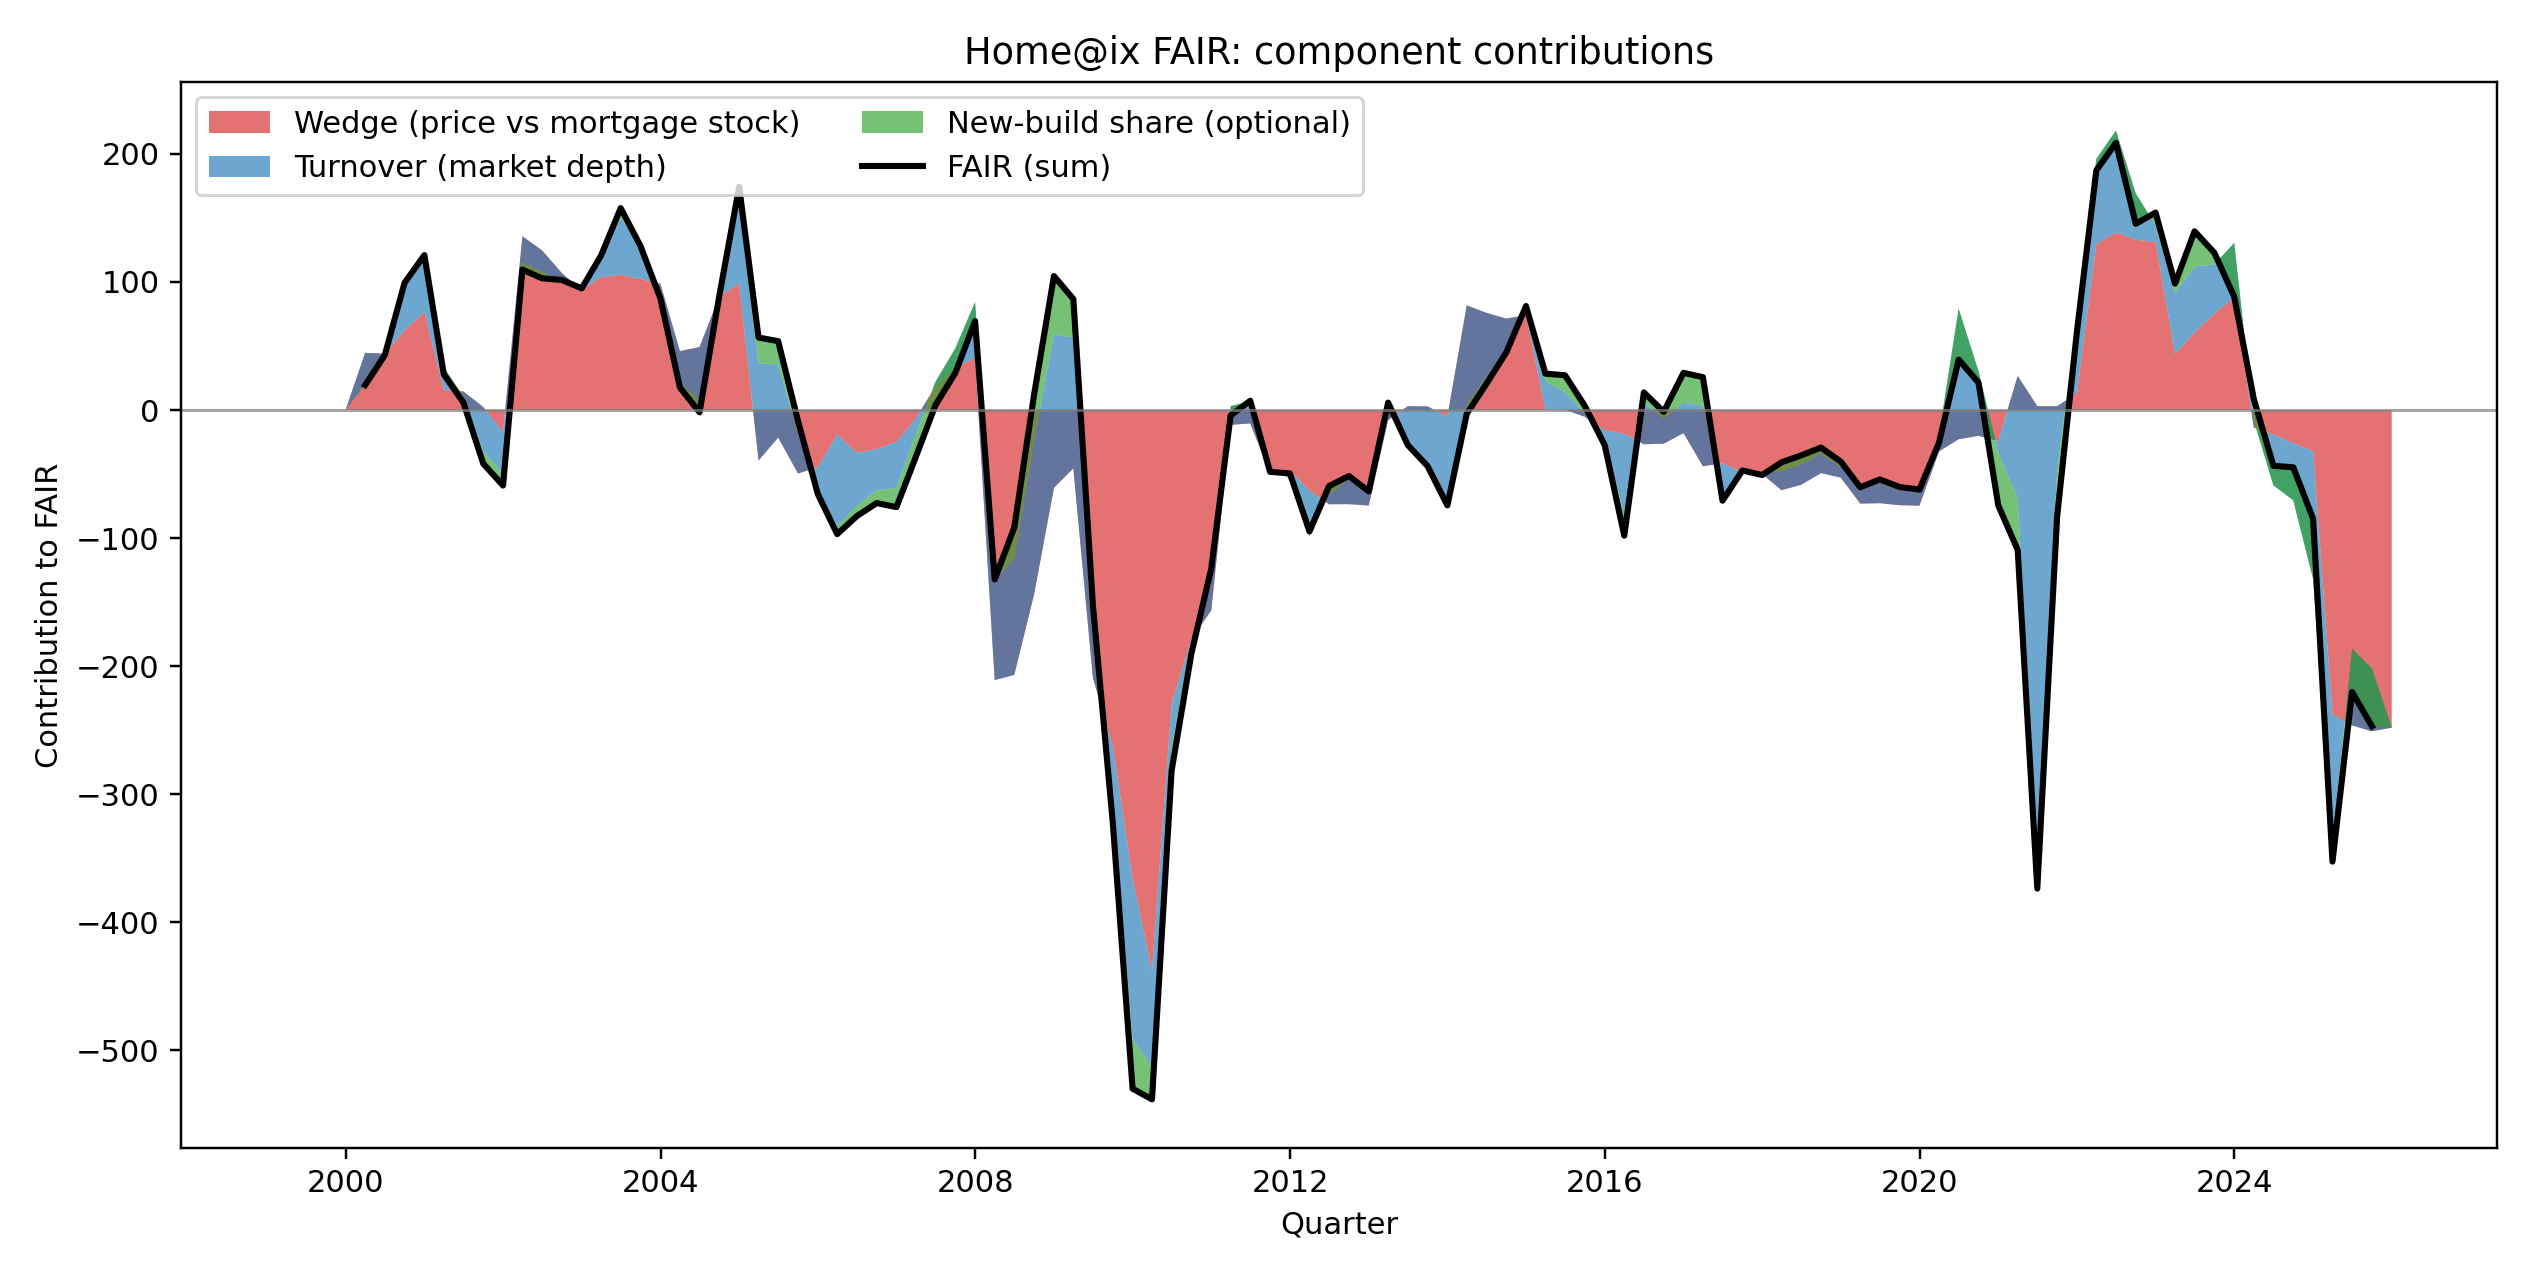
\includegraphics[width=0.95\textwidth]{fig_fair_contributions.png}
  \caption{Home@ix FAIR (EW): Component contributions. FAIR is the sum of wedge, turnover, and optional new-build terms.}
  \label{fig:fair_contrib}
\end{figure}

\section{Limitations and Extensions}
FAIR is a reduced-form indicator derived from aggregate market series. It does not directly encode distributional constraints (income heterogeneity, cash-buyer share, arrears microdata) or direct developer pacing series (e.g., sales per outlet per week) unless explicitly added. These are natural extensions; the baseline FAIR specification is intentionally reproducible and captures two dominant UK mechanisms: credit--price decoupling and thin-market clearing.

\section{Conclusion}
UK housing affordability is not only a price level problem; it is also an allocation and throughput problem. Home@ix FAIR provides a transparent, reproducible way to detect when the system is shifting into a regime where affordability is likely to deteriorate over a 2--3 year horizon via credit--price decoupling and/or collapsing market depth. Combined with direction-of-flow and event backtesting, FAIR is positioned as an operational forward-looking tool: a single ``Number'' grounded in auditable data and interpretable mechanisms.

\section*{Reproducibility Note}
The figures referenced in Section 8 are produced by the FAIR build scripts in the Home@ix workflow.

For the PDF build, the publication directory should contain (or be populated with) the following under \texttt{assets/fair/}:
\begin{itemize}
  \item \texttt{fig\_fair\_level.png}
  \item \texttt{fig\_fair\_contributions.png}
\end{itemize}

The FAIR output directory (from the build scripts) may also include:
\begin{itemize}
  \item \texttt{fair\_quarterly\_audit.csv}
  \item \texttt{anim\_fair\_direction\_of\_flow.gif} (note: GIF is not embedded in PDF; convert to PNG/MP4 for print/publication)
\end{itemize}

\end{document}
